\label{sec:supplementary}


\subsection*{Model Implementation details}
\label{sebsec:implementation_details}
Here are the implementation details.
%\subsubsection*{Large receptive field}
%
%% Please add the following required packages to your document preamble:
%% \usepackage{booktabs}
%\begin{table}[H]
%\begin{tabular}{@{}cccc@{}}\toprule
%\multicolumn{4}{c}{\textbf{ResNet50 Test Accuracy}}                                            \\ \midrule
%\textbf{Receptive Field} & \textbf{Dense}  & \textbf{Pruned (One Shot)} & \textbf{Difference In Accuracy} \\ \midrule
%1415                     & 32.00$\pm$0.192 & 32.00$\pm$0.192 & 0.000$\pm$0.000                 \\
%1920                     & 29.28$\pm$0.627 & 29.28$\pm$0.627 & 0.000$\pm$0.000                 \\
%3100                     & 22.84$\pm$0.370 & 22.84$\pm$0.370 & 0.000$\pm$0.000                 \\ \bottomrule
%\end{tabular}
%\caption{ReseNet50 with large Receptive Field on Tiny ImageNet  with pruning rate of 0.9}
%\label{tab:tiny imagenet largeRF one shot pruning rate 09}
%\end{table}
%\textbf{Large receptive field for CIFAR10}
%% Please add the following required packages to your document preamble:
%% \usepackage{booktabs}
%\begin{table}[H]
%\begin{tabular}{@{}cccc@{}}
%\toprule
%\multicolumn{4}{c}{\textbf{ResNet50 Accuracy}}                                                                                         \\ \midrule
%\textbf{Receptive Field} & \textbf{Dense}  & \multicolumn{1}{l}{\textbf{Pruned ( One Shot)}} & \multicolumn{1}{l}{\textbf{Difference in Accuracy}} \\ \midrule
%1415                     & 72.87$\pm$0.787 & 72.87$\pm$0.787                     & 0.000$\pm$0.000                                     \\
%1920                     & 53.37$\pm$1.293 & 53.37$\pm$1.293                     & 0.000$\pm$0.000                                     \\
%3100                     & 50.11$\pm$0.256 & 50.11$\pm$0.256                     & 0.000$\pm$0.000                                     \\ \bottomrule
%\end{tabular}
%\caption{ReseNet50 with large receptive field in CIFAR10}
%\label{tab:cifar10  largeRF one shot pruning rate 09}
%\end{table}
%
%\textbf{Width related experiments}
%
%% Please add the following required packages to your document preamble:
%% \usepackage{booktabs}
%% \usepackage{multirow}
%\begin{table}[H]
%\begin{tabular}{@{}cccc@{}}
%\toprule
%\textbf{Receptive Field} & \textbf{Width} & \textbf{Final Test Accuracy} & \multicolumn{1}{l}{\textbf{Original Test Accuracy}} \\ \midrule
%\multirow{2}{}{3100}    & $\times2$             & 26.33                        & \multirow{2}{}{22.84$\pm$0.370}                    \\
%                         & $\times3$             & 26.04                        
%                         \\ \bottomrule %\cmidrule(lr){2-3}
%\end{tabular}
%\caption{ReseNet50 with 2X and 3X width with receptive field of 3100 Tiny ImageNet }
%\label{tab:cifar10  largeRF one shot pruning rate 09}
%\end{table}
%
\subsection{One-shot Solutions with Multiple Pruning Rates}
\label{subsec:OneShotPruningRates}
For every combination 5 models were trained, pruned and fine-tuned. The error bars correspond to the standard deviation.

\textbf{Pruning Rate 0.8}
%\todo[inline]{All of the following figures would be better on tables}
% Please add the following required packages to your document preamble:
% \usepackage{booktabs}
\begin{table}[H]
  \centering
\begin{tabular}{@{}cccc@{}}
\toprule
\multicolumn{4}{c}{\textbf{VGG Accuracy}}                                                                                                                                  \\ \midrule
\textbf{Receptive Field} & \textbf{Dense} & \multicolumn{1}{l}{\textbf{Pruned} } & \multicolumn{1}{l}{\textbf{Difference In Accuracy}} \\ \midrule
181                      & 93.52$\pm$0.115              & 72.22$\pm$27.11                                   & 21.30$\pm$27.18                                     \\
359                      & 91.15$\pm$0.232              & 90.23$\pm$1.32                                    & 0.916$\pm$1.50                                      \\
537                      & 87.87$\pm$0.193              & 87.87$\pm$0.193                                   & 0.0\textbackslash{}pm\$0.0                          \\
715                      & 85.88$\pm$0.217              & 85.880$\pm$0.217                                  & 0.0$\pm$0.0                                         \\ \midrule
\multicolumn{4}{c}{\textbf{ResNet50}}                                                                                                                             \\ \midrule
\textbf{Receptive Field} & \textbf{Dense} & \textbf{Pruned}                     & \textbf{Difference In Accuracy}                     \\
110                      & 94.69$\pm$0.213              & 92.34$\pm$1.084                                   & 2.350$\pm$0.921                                     \\
213                      & 94.03$\pm$0.236              & 93.81$\pm$0.218                                   & 0.220$\pm$0.234                                     \\
318                      & 92.22$\pm$0.244              & 92.14$\pm$0.227                                   & 0.080$\pm$0.036                                     \\
423                      & 90.23$\pm$0.169              & 90.23$\pm$0.145                                   & -0.003$\pm$0.035                                    \\ \bottomrule
\end{tabular}
\caption{VGG and ResNet50 on CIFAR10 and pruning rate 0.8}
\label{tab:cifar10 pruning rate08}
\end{table}

% Please add the following required packages to your document preamble:
% \usepackage{booktabs}
\begin{table}[H]
  \centering
\begin{tabular}{@{}cccc@{}}
\toprule
\multicolumn{4}{c}{\textbf{VGG Accuracy}}                                                                                                                                  \\ \midrule
\textbf{Receptive Field} & \textbf{Dense} & \multicolumn{1}{l}{\textbf{Pruned}} & \multicolumn{1}{l}{\textbf{Difference In Accuracy}} \\ \midrule
181                      & 61.58$\pm$0.333              & 19.14$\pm$4.610                                   & 42.44$\pm$4.669                                     \\
359                      & 53.25$\pm$0.207              & 10.09$\pm$1.931                                   & 43.16$\pm$2.085                                     \\
537                      & 41.05$\pm$1.917              & 40.09$\pm$2.129                                   & 0.958$\pm$0.360                                     \\
715                      & 38.57$\pm$1.691              & 37.87$\pm$1.566                                   & 0.700$\pm$0.524                                     \\ \midrule
\multicolumn{4}{c}{\textbf{ResNet50 Accuracy}}                                                                                                                             \\ \midrule
\textbf{Receptive Field} & \textbf{Dense} & \textbf{Pruned}                     & \textbf{Difference In Accuracy}                     \\
213                      & 61.83$\pm$0.401              & 40.56$\pm$3.039                                   & 21.27$\pm$3.170                                     \\
318                      & 59.10$\pm$0.368              & 43.09$\pm$1.880                                   & 16.01$\pm$1.824                                     \\
423                      & 56.53$\pm$0.279              & 49.27$\pm$0.580                                   &
7.260$\pm$0.412                                     \\ \bottomrule \\
\end{tabular}
\caption{VGG and ResNet50 Tiny ImageNet pruning rate 0.8}
\label{tab:tiny imagenet pruning rate08}
\end{table}


%
%\begin{figure}[h]
% \centering
%     \begin{subfigure}[b]{\columnwidth}
%    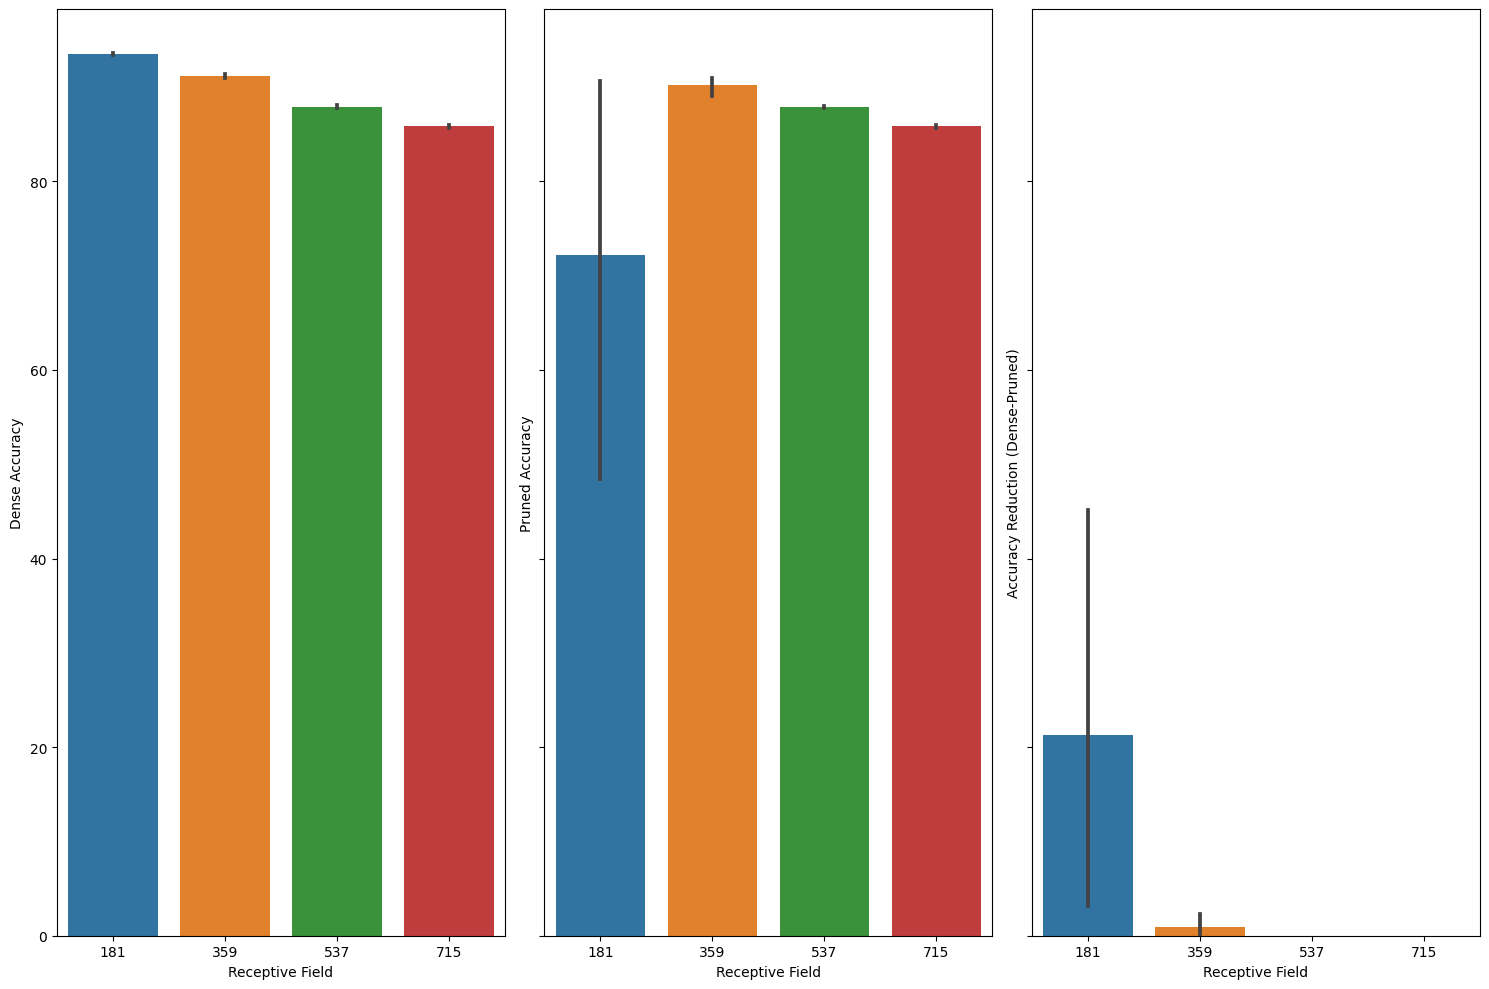
\includegraphics[width=1.1\columnwidth]{images/Supplementary_material/cifar10_vgg19_pruning_results_0.8.png}
%    \caption{VGG}
%    \label{subfig:vgg19CIfar10PR0.8}
%     \end{subfigure}
%      \hfill
%     \begin{subfigure}[b]{\columnwidth}
%    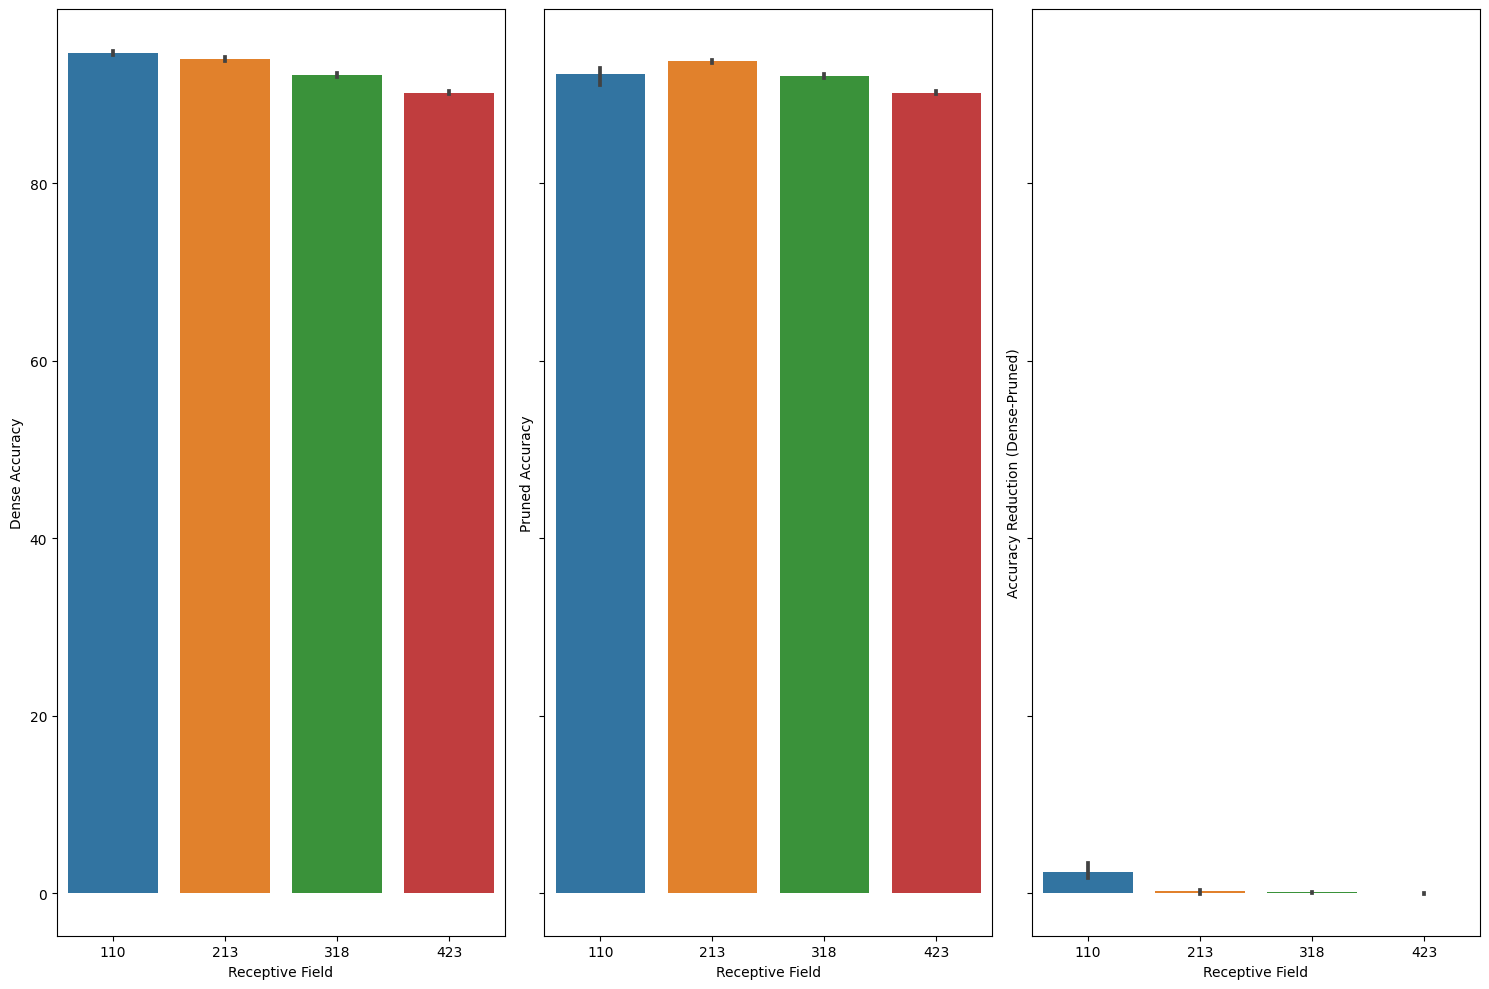
\includegraphics[width=1.1\columnwidth]{images/Supplementary_material/cifar10_resnet50_pruning_results_0.8.png}
%    \caption{ResNet-50}
%    \label{subfig:resenet50CIfar10PR0.8}
%     \end{subfigure}
%     \caption{ CIFAR10 pruning rate 0.8 results}
%    \label{fig:pr_0.8_CIFAR10}
%\end{figure}
%
%\begin{figure}[h]
% \centering
%     \begin{subfigure}[b]{\columnwidth}
%    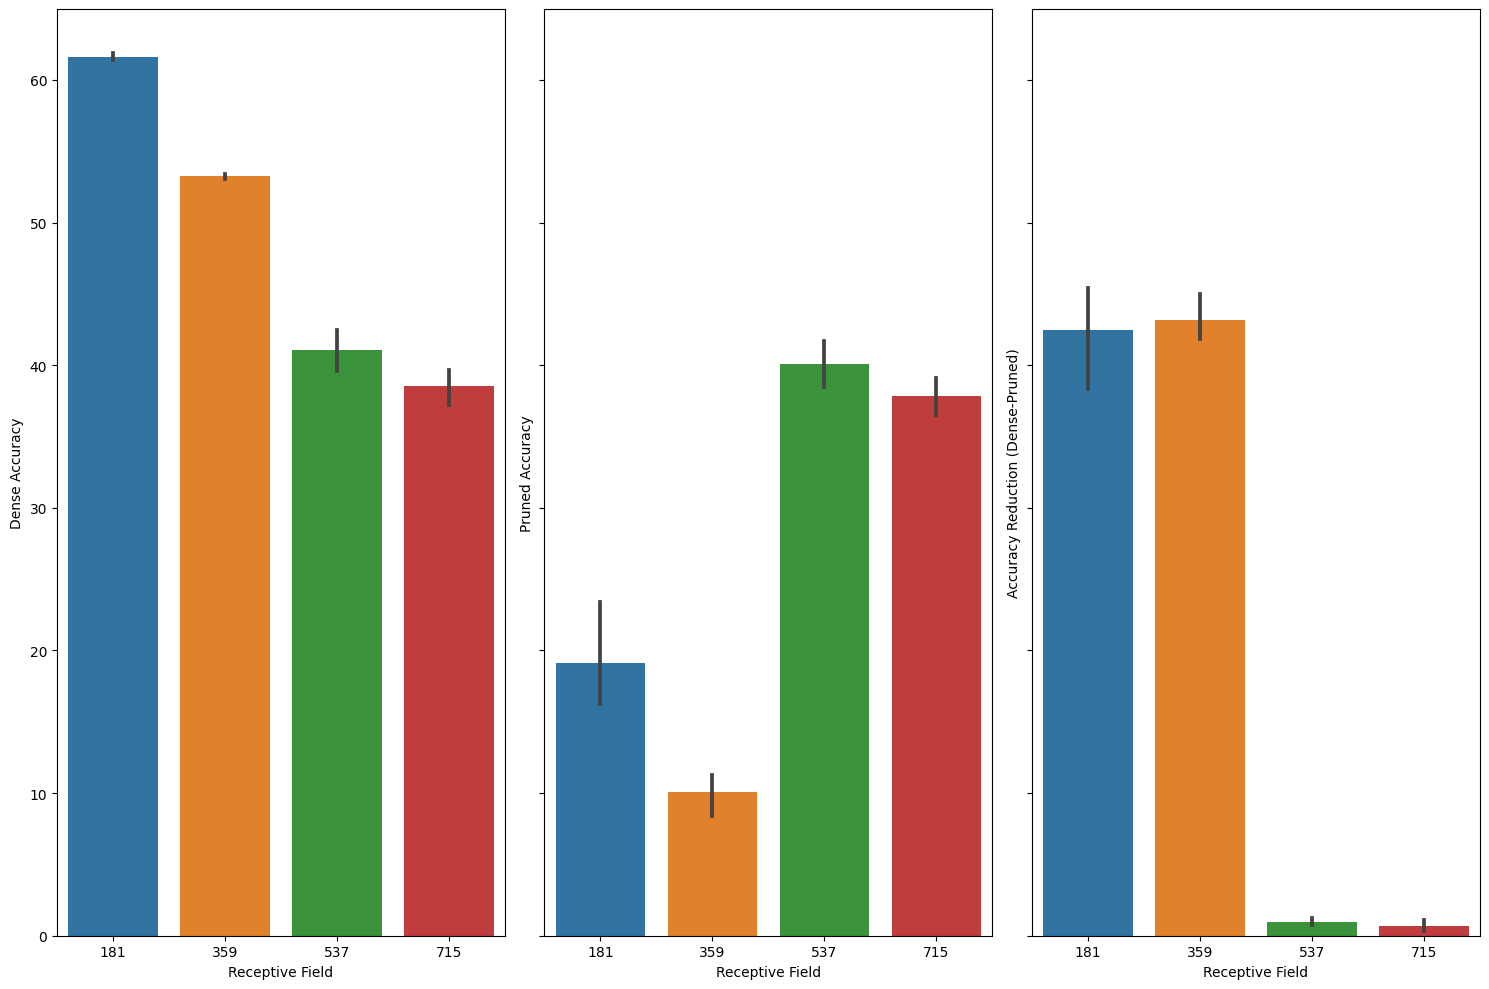
\includegraphics[width=1.1\columnwidth]{images/Supplementary_material/tiny_imagenet_vgg19_pruning_results_0.8.png}
%    \caption{VGG}
%    \label{subfig:vgg19CIfar10PR0.8}
%     \end{subfigure}
%      \hfill
%     \begin{subfigure}[b]{\columnwidth}
%    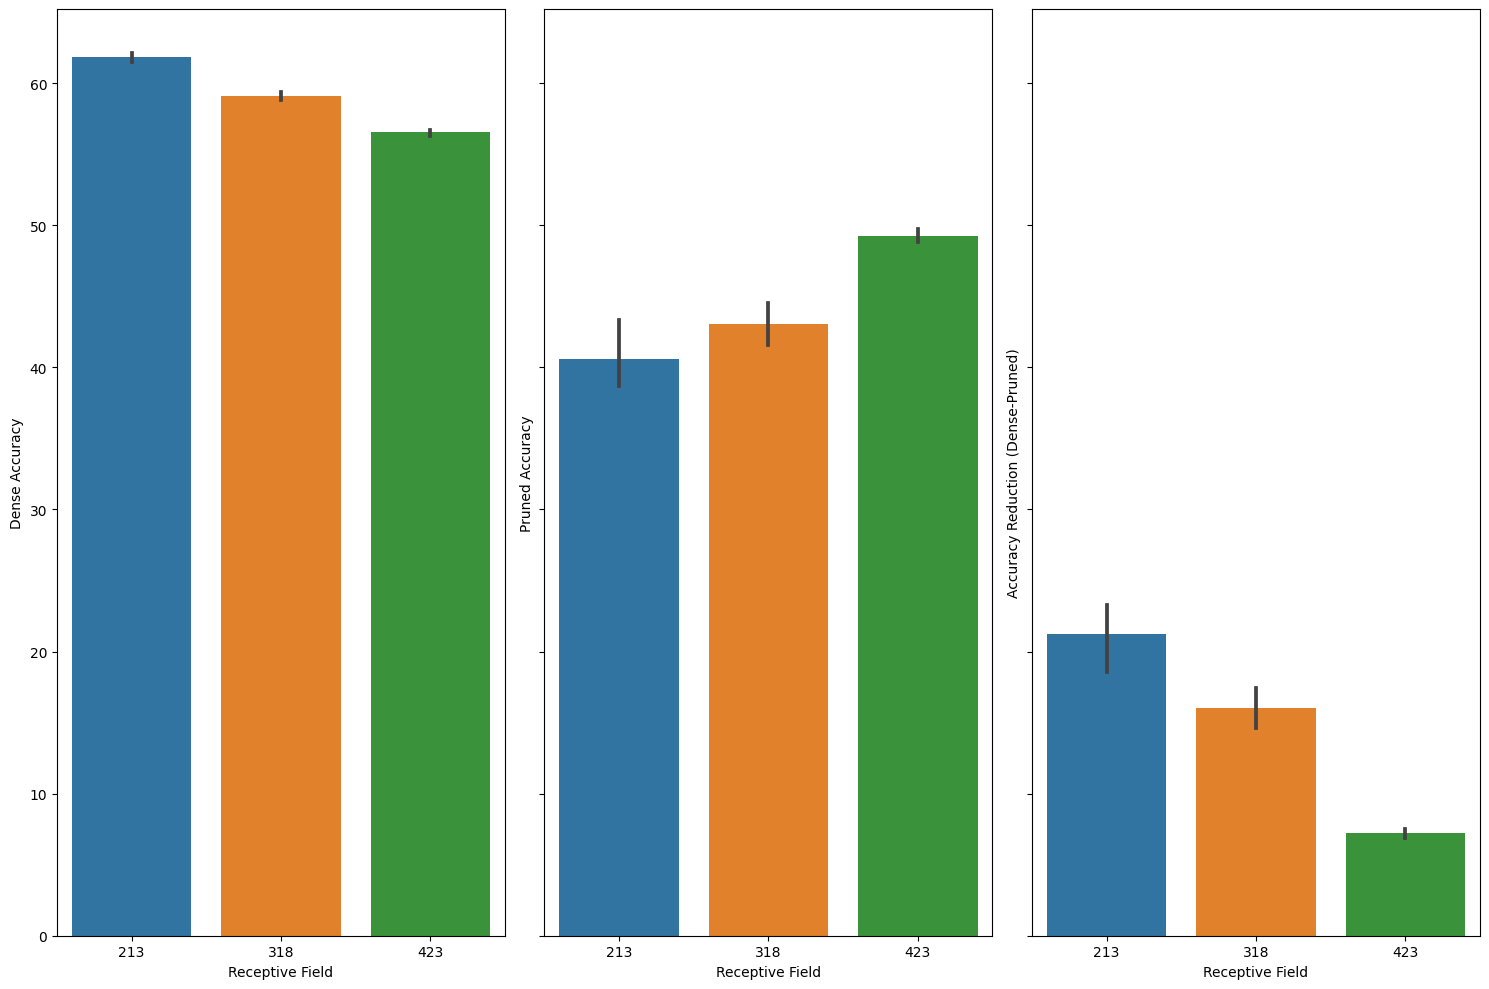
\includegraphics[width=1.1\columnwidth]{images/Supplementary_material/tiny_imagenet_resnet50_pruning_results_0.8.png}
%    \caption{ResNet-50}
%    \label{subfig:resenet50CIfar10PR0.8}
%     \end{subfigure}
%     \caption{ Tiny ImageNet pruning 0.8 results}
%    \label{fig:pr_0.8_tiny_imagenet}
%\end{figure}
%
\subsubsection*{Pruning Rate 0.7}
% Please add the following required packages to your document preamble:
% \usepackage{booktabs}
\begin{table}[H]
  \centering
\begin{tabular}{@{}cccc@{}}
\toprule
\multicolumn{4}{c}{\textbf{VGG Accuracy}}                                                                                                                                  \\ \midrule
\textbf{Receptive Field} & \textbf{Dense} & \multicolumn{1}{l}{\textbf{Pruned}} & \multicolumn{1}{l}{\textbf{Difference In Accuracy}} \\ \midrule
181                      & 93.52$\pm$0.115              & 93.32$\pm$0.104                                   & 0.206$\pm$0.155                                     \\
359                      & 91.15$\pm$0.232              & 91.10$\pm$0.230                                   & 0.058$\pm$0.050                                     \\
537                      & 87.88$\pm$0.193              & 87.88$\pm$0.193                                   & 0.0$\pm$0.0                                         \\
715                      & 85.88$\pm$0.217              & 85.88$\pm$0.217                                   & 0.0$\pm$0.0                                         \\ \midrule
\multicolumn{4}{c}{\textbf{ResNet50 Accuracy}}                                                                                                                             \\ \midrule
\textbf{Receptive Field} & \textbf{Dense} & \textbf{Pruned}                     & \textbf{Difference In Accuracy}                     \\
110                      & 94.69$\pm$0.213              & 94.24$\pm$0.204                                   & 0.453$\pm$0.012                                     \\
213                      & 94.03$\pm$0.236              & 93.93$\pm$0.203                                   & 0.097$\pm$0.093                                     \\
318                      & 92.22$\pm$0.244              & 92.24$\pm$0.254                                   & -0.020$\pm$0.010                                    \\
423                      & 90.23$\pm$0.169              & 90.23$\pm$0.175                                   &
-0.007$\pm$0.006                                    \\ \bottomrule \\
\end{tabular}
\caption{VGG and ResNet50 on CIFAR10 and pruning rate 0.7}
\label{tab:cifar10 pruning rate07}
\end{table}
% Please add the following required packages to your document preamble:
% \usepackage{booktabs}

\begin{table}[H]
  \centering
\begin{tabular}{@{}cccc@{}}
\toprule
\multicolumn{4}{c}{\textbf{VGG}}                                                                                                                                  \\ \midrule
\textbf{Receptive Field} & \textbf{Dense} & \multicolumn{1}{l}{\textbf{Pruned}} & \multicolumn{1}{l}{\textbf{Difference In Accuracy}} \\ \midrule
181                      & 61.58$\pm$0.333              & 48.29$\pm$1.390                                   & 13.29$\pm$1.462                                     \\
359                      & 53.25$\pm$0.207              & 40.02$\pm$2.558                                   & 13.23$\pm$2.646                                     \\
537                      & 41.05$\pm$1.917              & 40.96$\pm$1.934                                   & 0.092$\pm$0.070                                     \\
715                      & 38.57$\pm$1.691              & 38.51$\pm$1.658                                   & 0.068$\pm$0.087                                     \\ \midrule
\multicolumn{4}{c}{\textbf{ResNet50}}                                                                                                                             \\ \midrule
\textbf{Receptive Field} & \textbf{Dense} & \textbf{Pruned}                     & \textbf{Difference In Accuracy}                     \\
213                      & 61.83$\pm$0.401              & 55.33$\pm$0.987                                   & 6.504$\pm$1.194                                     \\
318                      & 59.10$\pm$0.368              & 54.28$\pm$0.398                                   & 4.816$\pm$0.319                                     \\
423                      & 56.53$\pm$0.279              & 54.41$\pm$0.449                                   &
2.128$\pm$0.216                                     \\ \bottomrule \\
\end{tabular}
\caption{VGG and ResNet50 on Tiny ImageNet and pruning rate 0.7}
\label{tab:tiny imagenet pruning rate07}
\end{table}

%
%\begin{figure}[h]
% \centering
%     \begin{subfigure}[b]{\columnwidth}
%    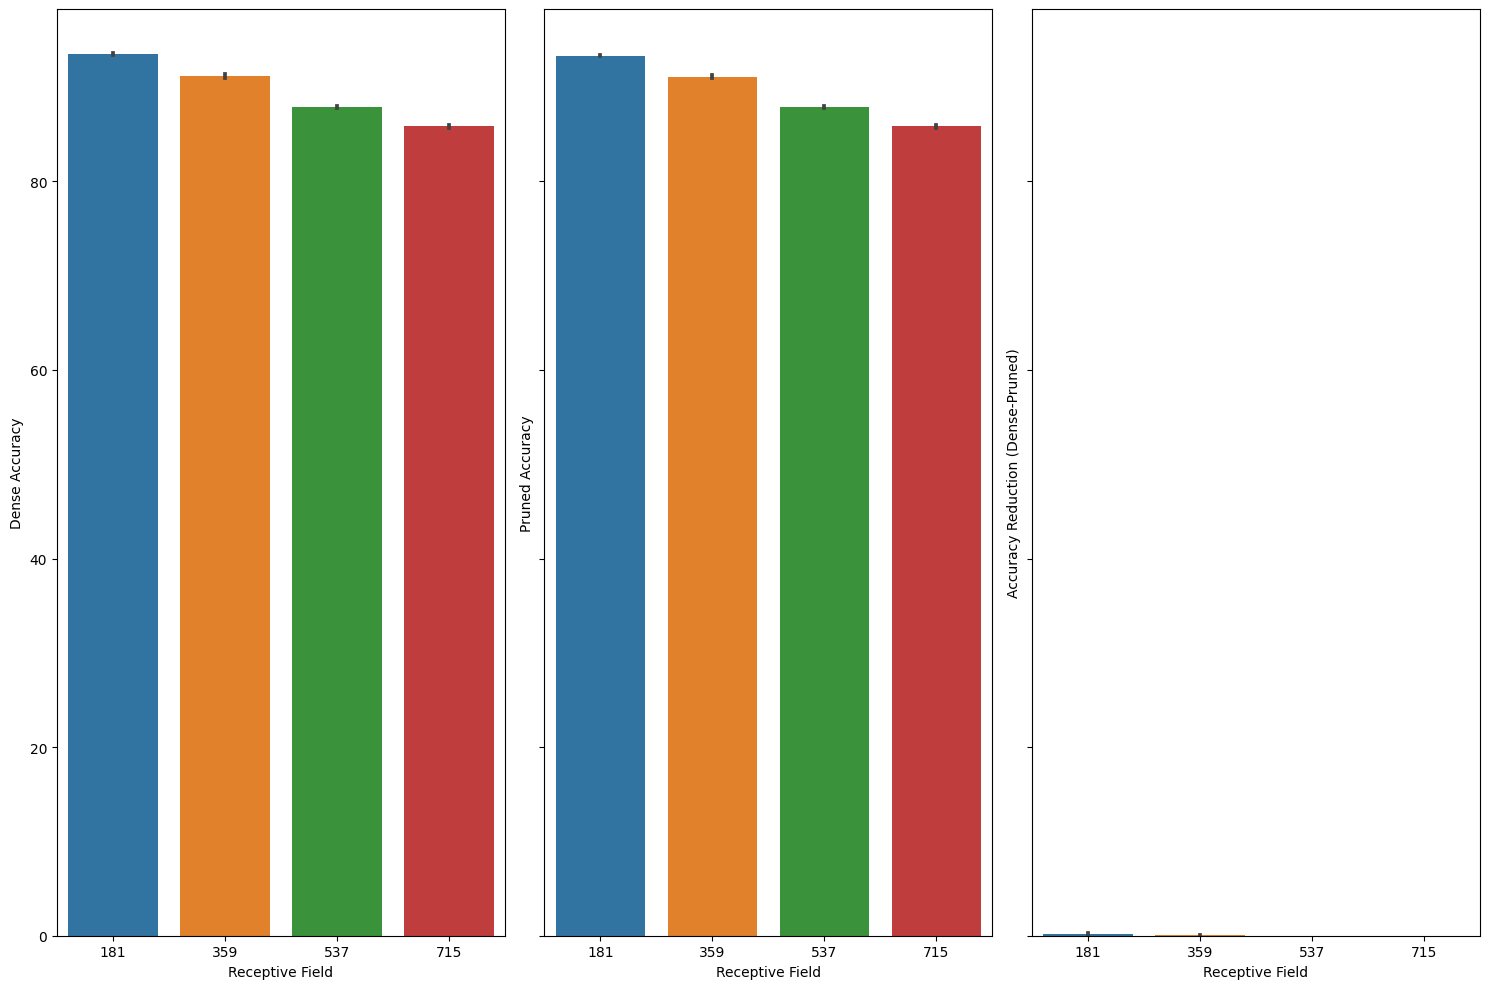
\includegraphics[width=1.1\columnwidth]{images/Supplementary_material/cifar10_vgg19_pruning_results_0.7.png}
%    \caption{VGG}
%    \label{subfig:vgg19CIfar10PR0.7}
%     \end{subfigure}
%      \hfill
%     \begin{subfigure}[b]{\columnwidth}
%    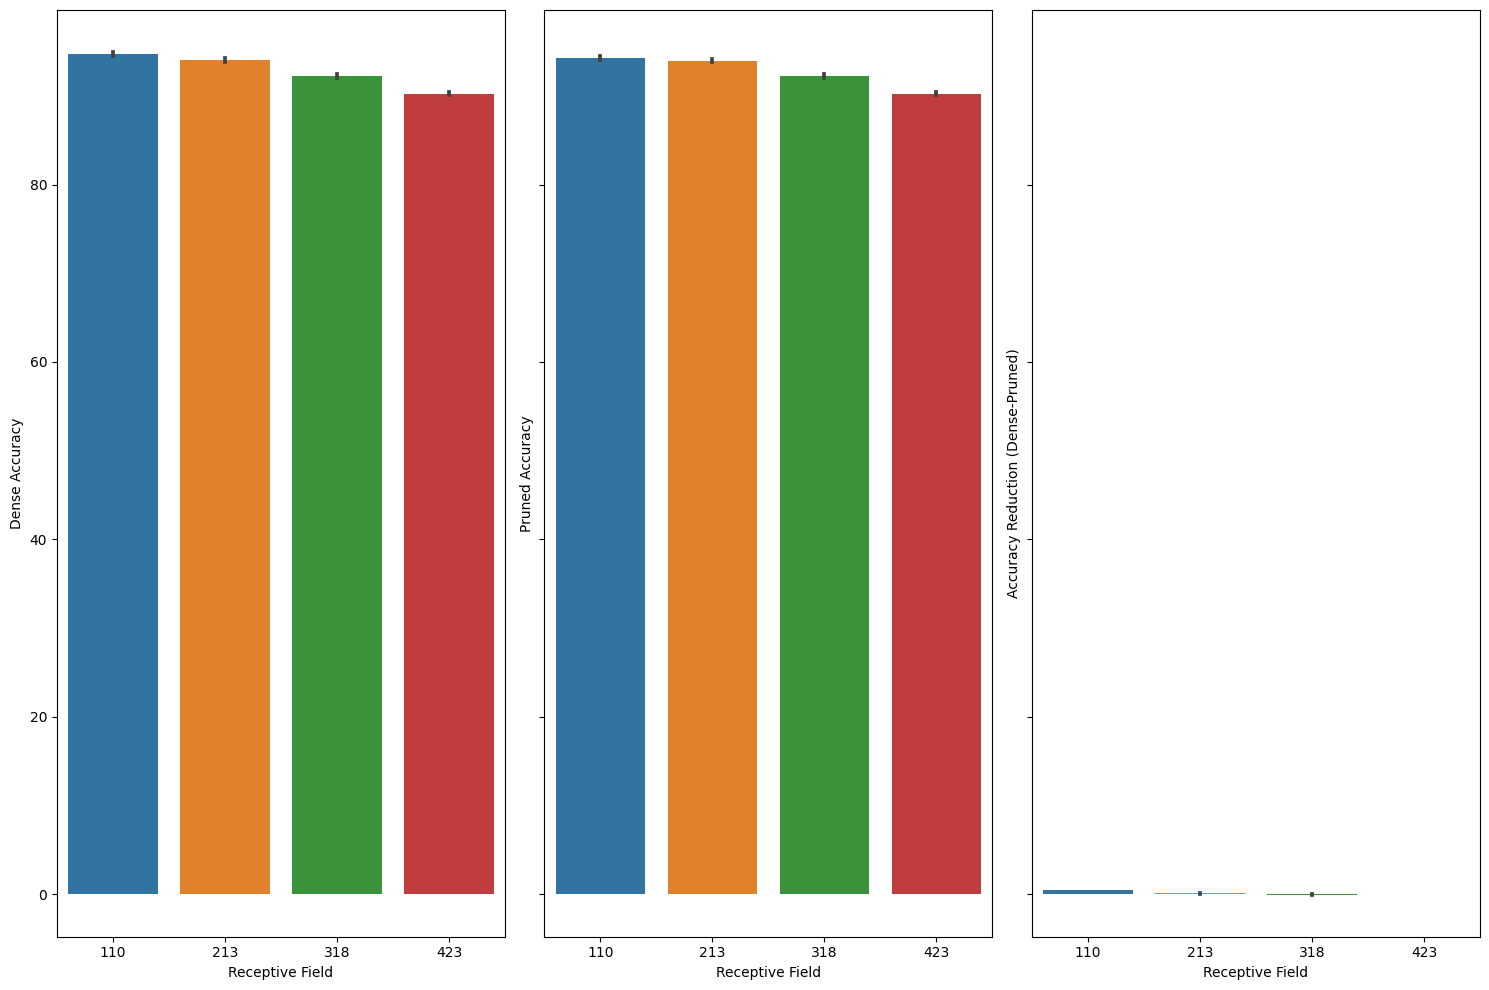
\includegraphics[width=1.1\columnwidth]{images/Supplementary_material/cifar10_resnet50_pruning_results_0.7.png}
%    \caption{ResNet-50}
%    \label{subfig:resenet50CIfar10PR0.7}
%     \end{subfigure}
%     \caption{ CIFAR10 0.7 results}
%    \label{fig:pr_0.7_CIFAR10}
%\end{figure}
%
%
%\begin{figure}[h]
% \centering
%     \begin{subfigure}[b]{\columnwidth}
%    \includegraphics[width=1.1\columnwidth]{images/Supplementary_material/tiny_imagenet_vgg19_pruning_results_0.7.png}
%    \caption{VGG}
%    \label{subfig:vgg19CIfar10PR0.7}
%     \end{subfigure}
%      \hfill
%     \begin{subfigure}[b]{\columnwidth}
%    \includegraphics[width=1.1\columnwidth]{images/Supplementary_material/tiny_imagenet_resnet50_pruning_results_0.7.png}
%    \caption{ResNet-50}
%    \label{subfig:resenet50CIfar10PR0.7}
%     \end{subfigure}
%     \caption{ Tiny ImageNet pruning 0.7 results}
%    \label{fig:pr_0.7_tiny_imagenet}
%\end{figure}
%
%
\subsubsection*{Pruning Rate 0.6}

% Please add the following required packages to your document preamble:
% \usepackage{booktabs}
\begin{table}[H]
  \centering
\begin{tabular}{@{}cccc@{}}
\toprule
\multicolumn{4}{c}{\textbf{VGG Accuracy}}                                                                                                                                  \\ \midrule
\textbf{Receptive Field} & \textbf{Dense} & \multicolumn{1}{l}{\textbf{Pruned}} & \multicolumn{1}{l}{\textbf{Difference In Accuracy}} \\ \midrule
181                      & 93.52$\pm$0.115              & 93.48$\pm$0.109                                   & 0.048$\pm$0.050                                     \\
359                      & 91.15$\pm$0.232              & 91.15$\pm$0.240                                   & 0.004$\pm$0.015                                     \\
537                      & 87.88$\pm$0.193              & 87.88$\pm$0.193                                   & 0.000$\pm$0.000                                     \\
715                      & 85.88$\pm$0.217              & 85.88$\pm$0.217                                   & 0.000$\pm$0.000                                     \\ \midrule
\multicolumn{4}{c}{\textbf{ResNet50 Accuracy}}                                                                                                                             \\ \midrule
\textbf{Receptive Field} & \textbf{Dense} & \textbf{Pruned}                     & \textbf{Difference In Accuracy}                     \\
110                      & 94.69$\pm$0.213              & 94.61$\pm$0.190                                   & 0.080$\pm$0.026                                     \\
213                      & 94.03$\pm$0.236              & 94.01$\pm$0.234                                   & 0.020$\pm$0.020                                     \\
318                      & 92.22$\pm$0.244              & 92.23$\pm$0.225                                   & -0.010$\pm$0.020                                    \\
423                      & 90.23$\pm$0.169              & 90.23$\pm$0.169                                   &
0.000$\pm$0.000                                     \\ \bottomrule \\
\end{tabular}
\caption{VGG and ResNet50 CIFAR10 pruning rate 0.6}
\label{tab:cifar10 pruning rate06}
\end{table}




% Please add the following required packages to your document preamble:
% \usepackage{booktabs}
\begin{table}[H]
  \centering
\begin{tabular}{@{}cccc@{}}
\toprule
\multicolumn{4}{c}{\textbf{VGG  Accuracy}}                                                                                                                                  \\ \midrule
\textbf{Receptive Field} & \textbf{Dense} & \multicolumn{1}{l}{\textbf{Pruned}} & \multicolumn{1}{l}{\textbf{Difference In Accuracy}} \\ \midrule
181                      & 61.58$\pm$0.333              & 56.93$\pm$0.512                                   & 4.656$\pm$0.663                                     \\
359                      & 53.25$\pm$0.207              & 47.94$\pm$1.896                                   & 5.304$\pm$1.963                                     \\
537                      & 41.05$\pm$1.917              & 41.05$\pm$1.913                                   & -0.000$\pm$0.071                                    \\
715                      & 38.57$\pm$1.691              & 38.58$\pm$1.659                                   & -0.008$\pm$0.039                                    \\ \midrule
\multicolumn{4}{c}{\textbf{ResNet50 Accuracy}}                                                                                                                             \\ \midrule
\textbf{Receptive Field} & \textbf{Dense} & \textbf{Pruned}                     & \textbf{Difference In Accuracy}                     \\
213                      & 61.83$\pm$0.401              & 59.28$\pm$0.468                                   & 2.552$\pm$0.489                                     \\
318                      & 59.10$\pm$0.368              & 57.26$\pm$0.467                                   & 1.840$\pm$0.356                                     \\
423                      & 56.53$\pm$0.279              & 55.97$\pm$0.459                                   &
0.568$\pm$0.212                                     \\ \bottomrule \\
\end{tabular}
\caption{VGG and ResNet50 Tiny ImageNet pruning rate 0.6}
\label{tab:tiny imagenet pruning rate06}
\end{table}





%
%\begin{figure}[h]
% \centering
%     \begin{subfigure}[b]{\columnwidth}
%    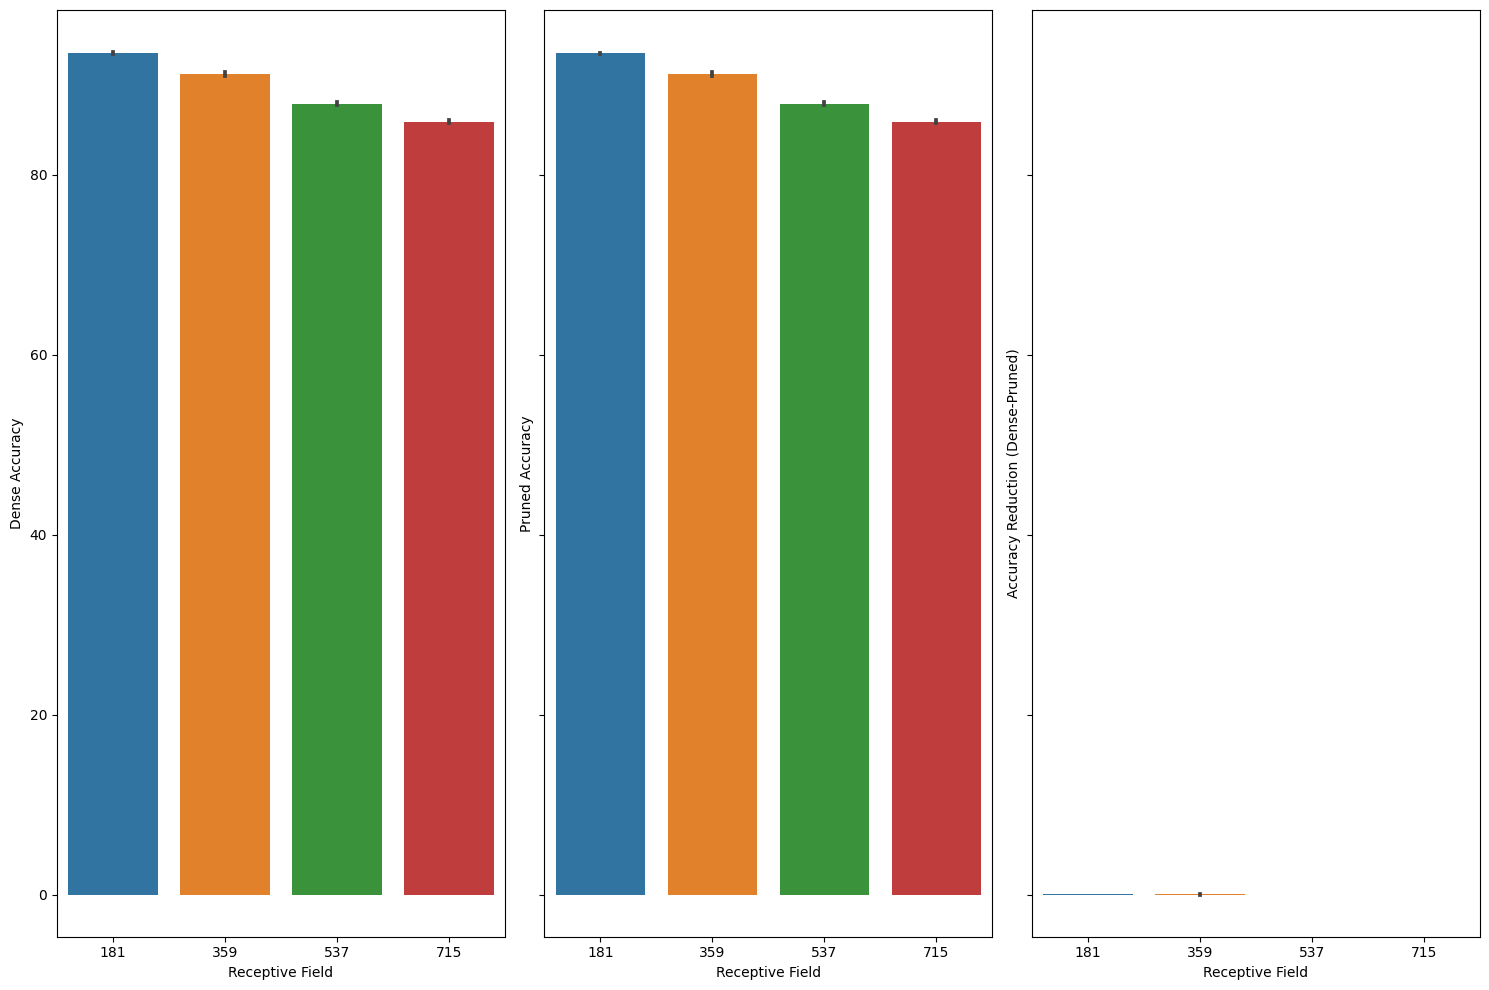
\includegraphics[width=1.1\columnwidth]{images/Supplementary_material/cifar10_vgg19_pruning_results_0.6.png}
%    \caption{VGG}
%    \label{subfig:vgg19CIfar10PR0.6}
%     \end{subfigure}
%      \hfill
%     \begin{subfigure}[b]{\columnwidth}
%    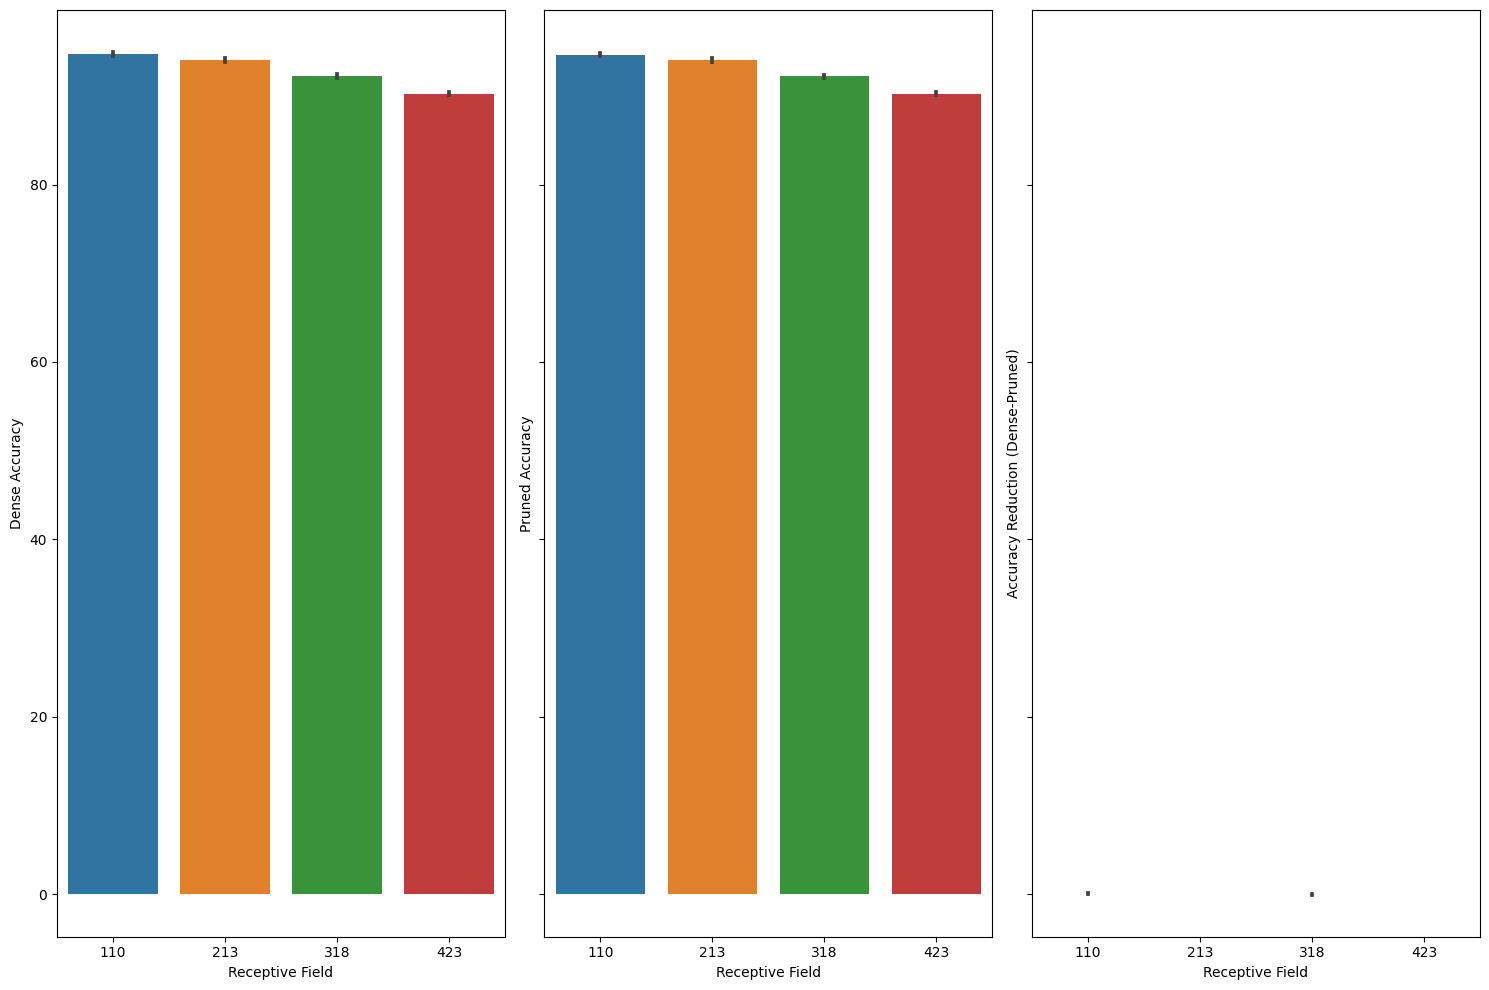
\includegraphics[width=1.1\columnwidth]{images/Supplementary_material/cifar10_resnet50_pruning_results_0.6.png}
%    \caption{ResNet-50}
%    \label{subfig:resenet50CIfar10PR0.6}
%     \end{subfigure}
%     \caption{ CIFAR10 0.6 results}
%    \label{fig:pr_0.7_CIFAR10}
%\end{figure}
%
%
%\begin{figure}[h]
% \centering
%     \begin{subfigure}[b]{\columnwidth}
%    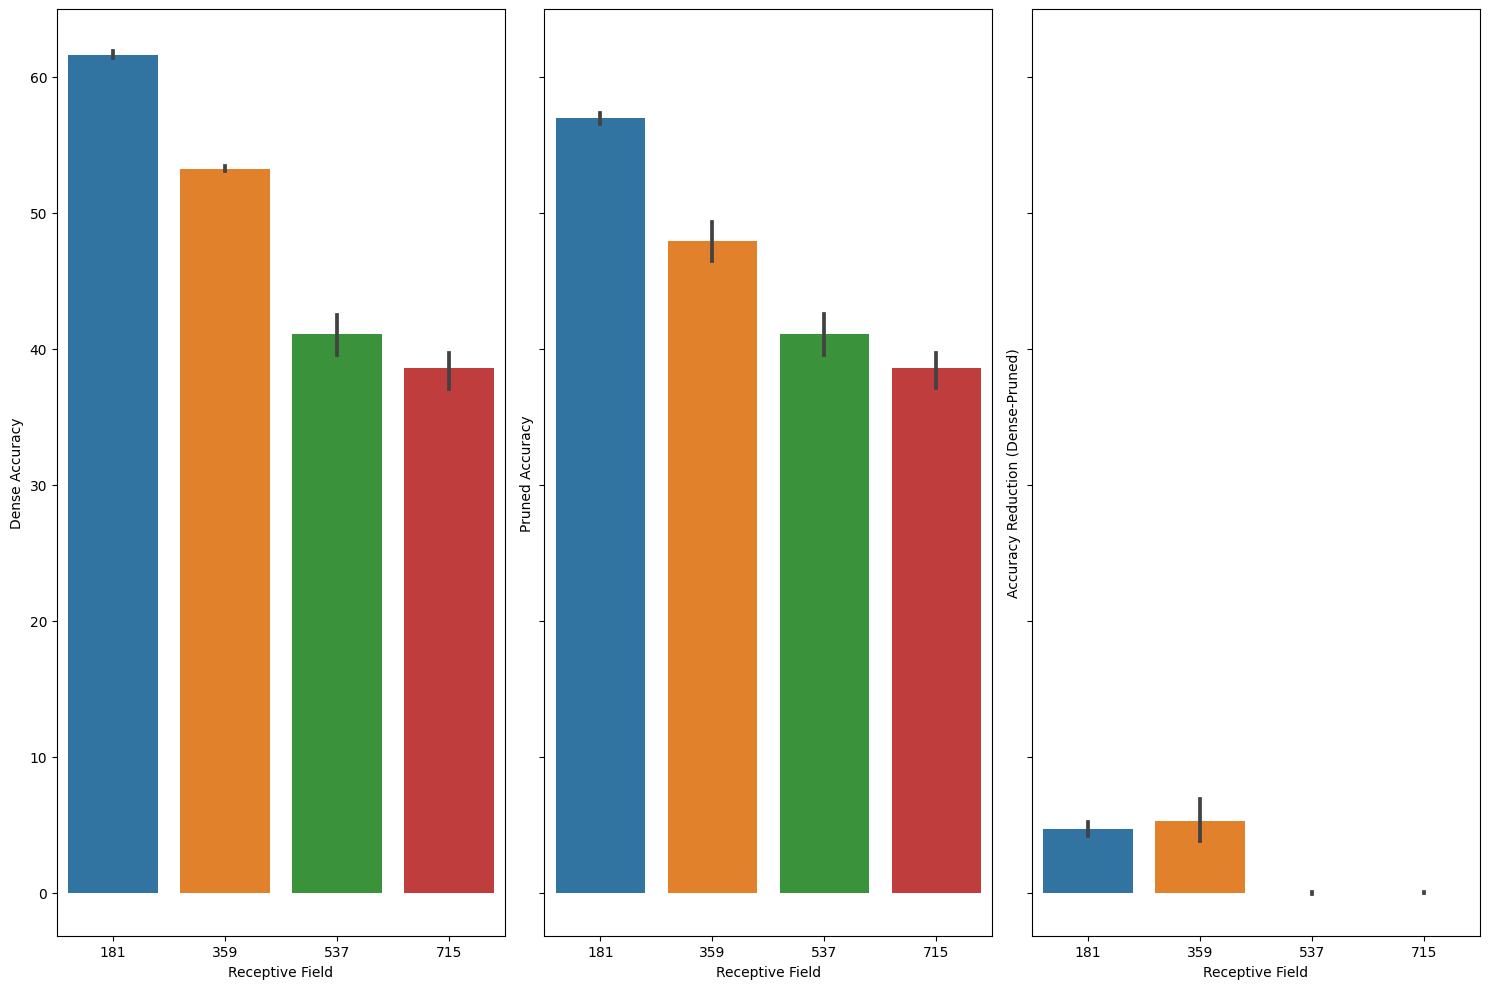
\includegraphics[width=1.1\columnwidth]{images/Supplementary_material/tiny_imagenet_vgg19_pruning_results_0.6.png}
%    \caption{VGG}
%    \label{subfig:vgg19CIfar10PR0.6}
%     \end{subfigure}
%      \hfill
%     \begin{subfigure}[b]{\columnwidth}
%    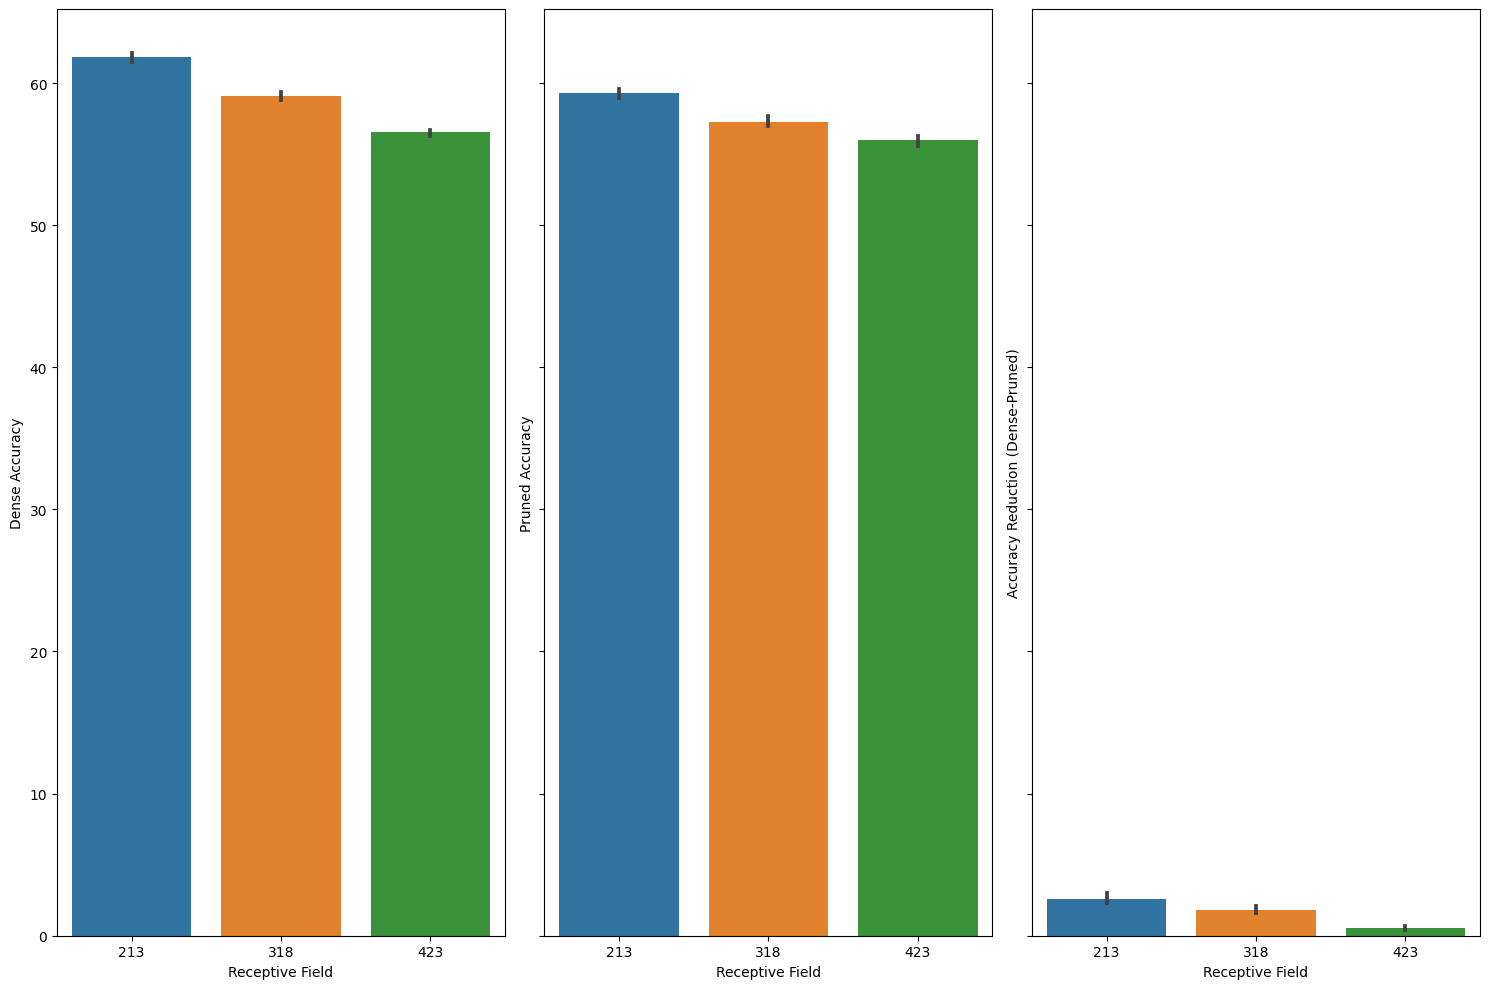
\includegraphics[width=1.1\columnwidth]{images/Supplementary_material/tiny_imagenet_resnet50_pruning_results_0.6.png}
%    \caption{ResNet-50}
%    \label{subfig:resenet50CIfar10PR0.6}
%     \end{subfigure}
%     \caption{ Tiny ImageNet 0.6 results}
%
%    \label{fig:pr_0.6_tiny_imagenet}
%
%\end{figure}
%
\subsubsection*{Pruning Rate 0.5}
% Please add the following required packages to your document preamble:
% \usepackage{booktabs}
\begin{table}[H]
  \centering
\begin{tabular}{@{}cccc@{}}
\toprule
\multicolumn{4}{c}{\textbf{VGG Accuracy}}                                                                                                                                  \\ \midrule
\textbf{Receptive Field} & \textbf{Dense} & \multicolumn{1}{l}{\textbf{Pruned}} & \multicolumn{1}{l}{\textbf{Difference In Accuracy}} \\ \midrule
181                      & 93.52$\pm$0.115              & 93.51$\pm$0.128                                   & 0.010$\pm$0.029                                     \\
359                      & 91.15$\pm$0.232              & 91.16$\pm$0.237                                   & -0.004$\pm$0.005                                    \\
537                      & 87.88$\pm$0.193              & 87.88$\pm$0.193                                   & 0.000$\pm$0.000                                     \\
715                      & 85.88$\pm$0.217              & 85.88$\pm$0.217                                   & 0.000$\pm$0.000                                     \\ \midrule
\multicolumn{4}{c}{\textbf{ResNet50 Accuracy}}                                                                                                                             \\ \midrule
\textbf{Receptive Field} & \textbf{Dense} & \textbf{Pruned}                     & \textbf{Difference In Accuracy}                     \\
110                      & 94.69$\pm$0.213              & 94.71$\pm$0.202                                   & -0.023$\pm$0.012                                    \\
213                      & 94.03$\pm$0.236              & 94.02$\pm$0.243                                   & 0.010$\pm$0.026                                     \\
318                      & 92.22$\pm$0.244              & 92.22$\pm$0.229                                   & -0.003$\pm$0.015                                    \\
423                      & 90.23$\pm$0.169              & 90.23$\pm$0.169                                   &
0.000$\pm$0.000                                     \\ \bottomrule \\
\end{tabular}
\caption{VGG and ResNet50 on CIFAR10 with pruning rate 0.5}
\label{tab:cifar10 pruning rate05}
\end{table}
% Please add the following required packages to your document preamble:
% \usepackage{booktabs}
\begin{table}[H]
  \centering
\begin{tabular}{@{}cccc@{}}
\toprule
\multicolumn{4}{c}{\textbf{VGG  Accuracy}}                                                                                                                                  \\ \midrule
\textbf{Receptive Field} & \textbf{Dense} & \multicolumn{1}{l}{\textbf{Pruned}} & \multicolumn{1}{l}{\textbf{Difference In Accuracy}} \\ \midrule
181                      & 61.58$\pm$0.333              & 59.85$\pm$0.241                                   & 1.738$\pm$0.240                                     \\
359                      & 53.25$\pm$0.207              & 51.13$\pm$0.665                                   & 2.116$\pm$0.735                                     \\
537                      & 41.05$\pm$1.917              & 41.05$\pm$1.915                                   & -0.004$\pm$0.018                                    \\
715                      & 38.57$\pm$1.691              & 38.57$\pm$1.686                                   & 0.008$\pm$0.013                                     \\ \midrule
\multicolumn{4}{c}{\textbf{ResNet50  Accuracy}}                                                                                                                             \\ \midrule
\textbf{Receptive Field} & \textbf{Dense} & \textbf{Pruned}                     & \textbf{Difference In Accuracy}                     \\
213                      & 61.83$\pm$0.401              & 60.86$\pm$0.458                                   & 0.966$\pm$0.400                                     \\
318                      & 59.10$\pm$0.368              & 58.46$\pm$0.510                                   & 0.640$\pm$0.401                                     \\
423                      & 56.53$\pm$0.279              & 56.29$\pm$0.408                                   &
0.248$\pm$0.180                                     \\ \bottomrule \\
\end{tabular}
\caption{VGG and ResNet50 Tiny ImageNet with pruning rate 0.5}
\label{tab:tiny imagenet pruning rate05}
\end{table}

%
%\begin{figure}[h]
% \centering
%     \begin{subfigure}[b]{\columnwidth}
%    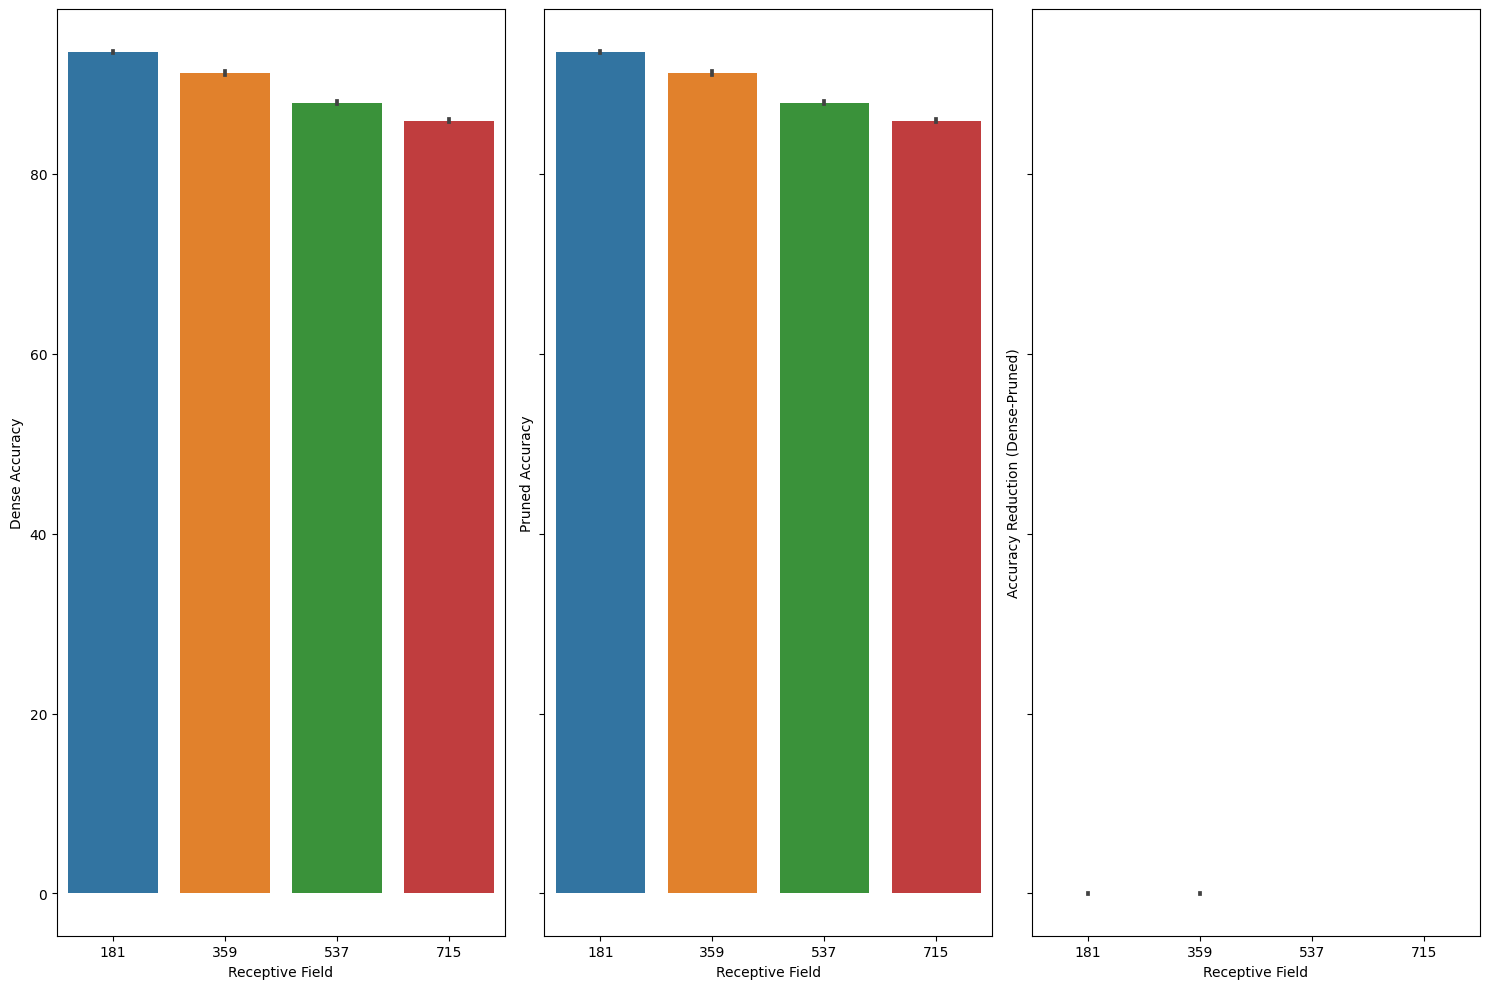
\includegraphics[width=1.1\columnwidth]{images/Supplementary_material/cifar10_vgg19_pruning_results_0.5.png}
%    \caption{VGG}
%    \label{subfig:vgg19CIfar10PR0.5}
%     \end{subfigure}
%      \hfill
%     \begin{subfigure}[b]{\columnwidth}
%    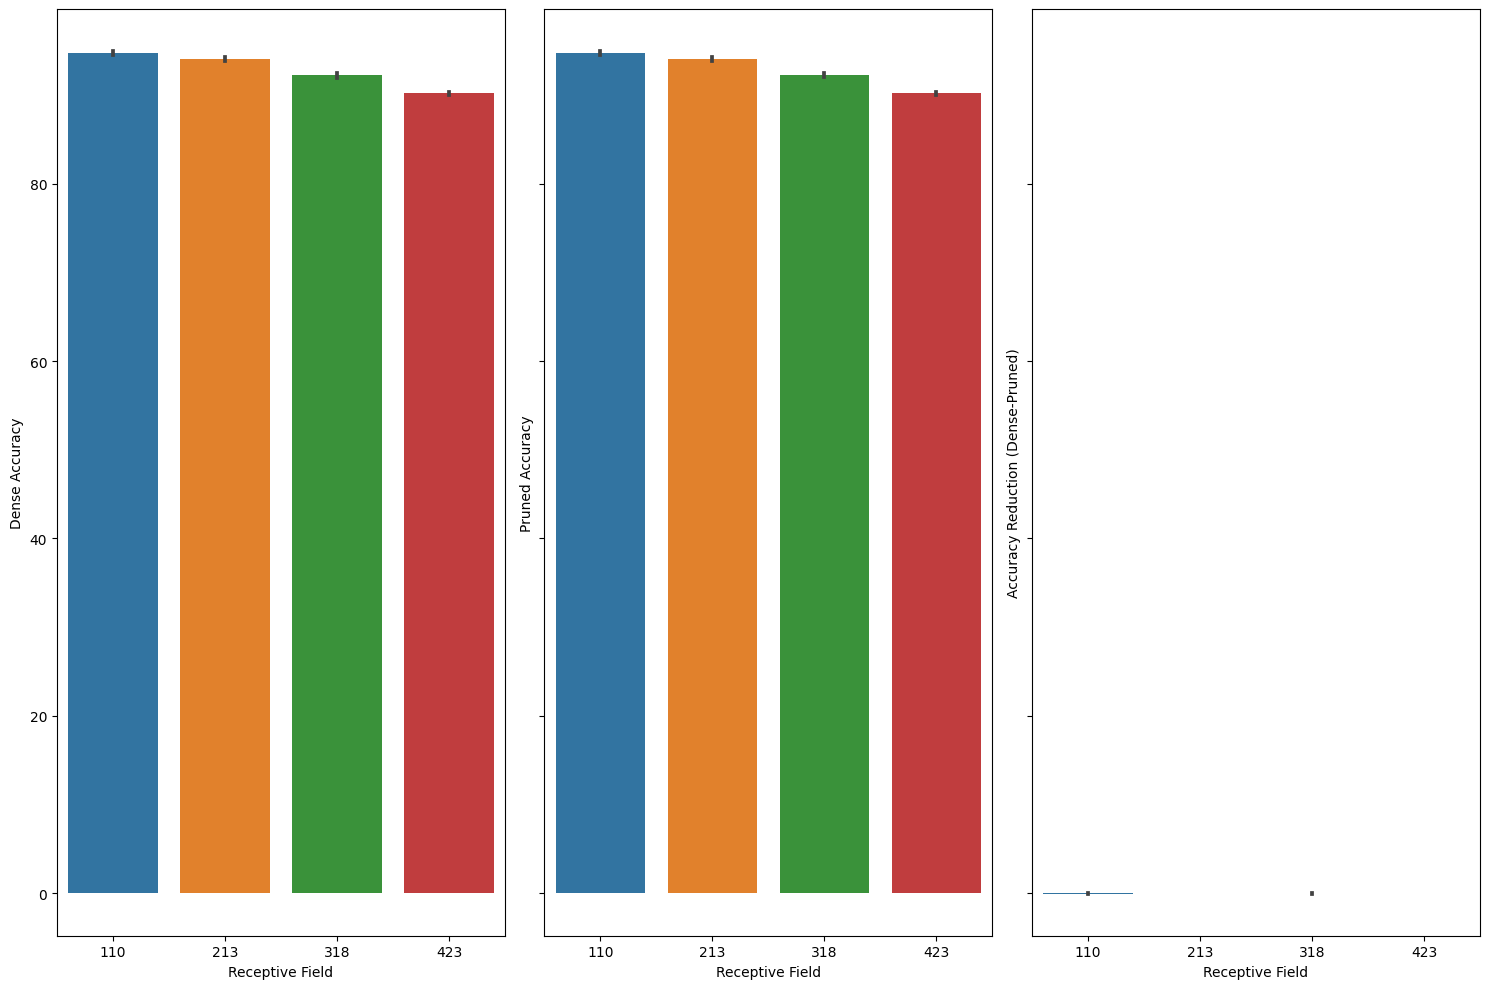
\includegraphics[width=1.1\columnwidth]{images/Supplementary_material/cifar10_resnet50_pruning_results_0.5.png}
%    \caption{ResNet-50}
%    \label{subfig:resenet50CIfar10PR0.5}
%     \end{subfigure}
%     \caption{ CIFAR10 0.5 results}
%    \label{fig:pr_0.5_CIFAR10}
%\end{figure}
%
%
%\begin{figure}[h]
% \centering
%     \begin{subfigure}[b]{\columnwidth}
%    \includegraphics[width=1.1\columnwidth]{images/Supplementary_material/tiny_imagenet_vgg19_pruning_results_0.5.png}
%    \caption{VGG}
%    \label{subfig:vgg19CIfar10PR0.5}
%     \end{subfigure}
%      \hfill
%     \begin{subfigure}[b]{\columnwidth}
%    \includegraphics[width=1.1\columnwidth]{images/Supplementary_material/tiny_imagenet_resnet50_pruning_results_0.5.png}
%    \caption{ResNet-50}
%    \label{subfig:resenet50CIfar10PR0.5}
%     \end{subfigure}
%     \caption{ Tiny ImageNet pruning 0.5 results}
%    \label{fig:pr_0.8_tiny_imagenet}
%\end{figure}
%


%################################## Fine tuned solutions ############################################################
%
%\subsection*{Fine-tuning pruned solutions}
%\label{subsec:Fine_tuning_solutions}
%Here we fine-tuned the pruned solutions while preserving the mask for 10 epochs with the following hyper-parameters
%\begin{itemize}
%  \item Initial Learning Rate: 0.0001,
%  \item Weight Decay:5e-4
%  \item Momentum:0,9
%  \item Gradient clip: 0.1
%\end{itemize}
%
%\todo[inline]{All of the following figures would be better on a table}
% Please add the following required packages to your document preamble:
% \usepackage{booktabs}
%
%\begin{table}[H]
%\begin{tabular}{@{}cccc@{}}
%\toprule
%\multicolumn{4}{c}{\textbf{VGG}}                                                                                                                                  \\ \midrule
%\textbf{Receptive Field} & \textbf{Dense Test Accuracy} & \multicolumn{1}{l}{\textbf{Pruned  TestAccuracy}} & \multicolumn{1}{l}{\textbf{Difference In Accuracy}} \\ \midrule
%181                      & 93.52$\pm$0.115              & 91.42$\pm$2.026                                   & 2.106$\pm$2.111                                     \\
%359                      & 91.15$\pm$0.232              & 90.81$\pm$0.293                                   & 0.348$\pm$0.366                                     \\
%537                      & 87.88$\pm$0.193              & 87.85$\pm$0.223                                   & 0.032$\pm$0.070                                     \\
%715                      & 85.88$\pm$0.217              & 85.78$\pm$0.286                                   & 0.096$\pm$0.140                                     \\ \midrule
%\multicolumn{4}{c}{\textbf{ResNet50}}                                                                                                                             \\ \midrule
%\textbf{Receptive Field} & \textbf{Dense Test Accuracy} & \textbf{Pruned  TestAccuracy}                     & \textbf{Difference In Accuracy}                     \\
%110                      & 94.69$\pm$0.213              & 90.86$\pm$0.701                                   & 3.830$\pm$0.795                                     \\
%213                      & 94.03$\pm$0.236              & 93.55$\pm$0.211                                   & 0.477$\pm$0.197                                     \\
%318                      & 92.22$\pm$0.244              & 92.03$\pm$0.200                                   & 0.190$\pm$0.053                                     \\
%423                      & 90.23$\pm$0.169              & 90.23$\pm$0.147                                   & -0.007$\pm$0.087                                    \\ \bottomrule
%\end{tabular}
%\caption{VGG and ResNet50 on CIFAR10 with fine tuning and pruning rate 0.9}
%\label{tab:cifar10 fine tuning pruning rate 09}
%\end{table}




%% Please add the following required packages to your document preamble:
%% \usepackage{booktabs}
%\begin{table}[H]
%\begin{tabular}{@{}cccc@{}}
%\toprule
%\multicolumn{4}{c}{\textbf{VGG}}                                                                                                                                  \\ \midrule
%\textbf{Receptive Field} & \textbf{Dense Test Accuracy} & \multicolumn{1}{l}{\textbf{Pruned  TestAccuracy}} & \multicolumn{1}{l}{\textbf{Difference In Accuracy}} \\ \midrule
%181                      & 61.58$\pm$0.333              & 30.21$\pm$2.595                                   & 31.37$\pm$2.534                                     \\
%359                      & 53.25$\pm$0.207              & 3.558$\pm$2.027                                   & 49.69$\pm$2.188                                     \\
%537                      & 41.05$\pm$1.917              & 38.21$\pm$2.699                                   & 2.842$\pm$0.884                                     \\
%715                      & 38.57$\pm$1.691              & 36.45$\pm$1.549                                   & 2.126$\pm$0.762                                     \\ \midrule
%\multicolumn{4}{c}{\textbf{ResNet50}}                                                                                                                             \\ \midrule
%\textbf{Receptive Field} & \textbf{Dense Test Accuracy} & \textbf{Pruned  TestAccuracy}                     & \textbf{Difference In Accuracy}                     \\
%213                      & 61.83$\pm$0.401              & 44.56$\pm$1.205                                   & 17.27$\pm$1.346                                     \\
%318                      & 59.10$\pm$0.368              & 44.28$\pm$0.648                                   & 14.82$\pm$0.633                                     \\
%423                      & 56.53$\pm$0.279              & 46.16$\pm$0.716                                   & 10.37$\pm$0.577                                     \\ \bottomrule
%\end{tabular}
%\caption{VGG and ReseNet50 on Tiny ImageNet with fine tuning  and pruning rate of 0.9}
%\label{tab:cifar10 fine tuning pruning rate 09}
%\end{table}


%\textbf{ Tiny ImageNet for 100 Epochs}







%% Please add the following required packages to your document preamble:
%% \usepackage{booktabs}
%\begin{table}[H]
%\begin{tabular}{@{}cccc@{}}
%\toprule
%\multicolumn{4}{c}{\textbf{VGG  Test Accuracy}}                                                                    \\ \midrule
%\textbf{Receptive Field} & \textbf{Dense}  & \textbf{Pruned} & \multicolumn{1}{l}{\textbf{Difference In Accuracy}} \\ \midrule
%181                      & 61.58$\pm$0.333 & 33.93$\pm$0.320 & 27.66$\pm$0.521                                     \\
%359                      & 53.25$\pm$0.207 & 29.73$\pm$16.15 & 23.52$\pm$16.23                                     \\
%537                      & 41.05$\pm$1.917 & 37.50$\pm$1.916 & 3.554$\pm$0.164                                     \\
%715                      & 38.57$\pm$1.691 & 35.50$\pm$1.812 & 3.078$\pm$0.453                                     \\ \midrule
%\multicolumn{4}{c}{\textbf{ResNet50 Test Accuracy}}                                                                \\ \midrule
%\textbf{Receptive Field} & \textbf{Dense}  & \textbf{Pruned} & \textbf{Difference In Accuracy}                     \\
%\midrule
%213                      & 61.83$\pm$0.401 & 50.21$\pm$0.428 & 11.62$\pm$0.487                                     \\
%318                      & 59.10$\pm$0.368 & 49.83$\pm$0.583 & 9.274$\pm$0.413                                     \\
%423                      & 56.53$\pm$0.279 & 49.43$\pm$0.403 & 7.106$\pm$0.361                                     \\ \bottomrule
%\end{tabular}
%\caption{VGG and ReseNet50 on Tiny ImageNet with fine tuning for 100 epochs and pruning rate of 0.9}
%\label{tab:tiny imagenet fine tuning pruning rate 09}
%\end{table}
%

%\begin{figure}[!htb]
% \centering
%     \begin{subfigure}[b]{\columnwidth}
%    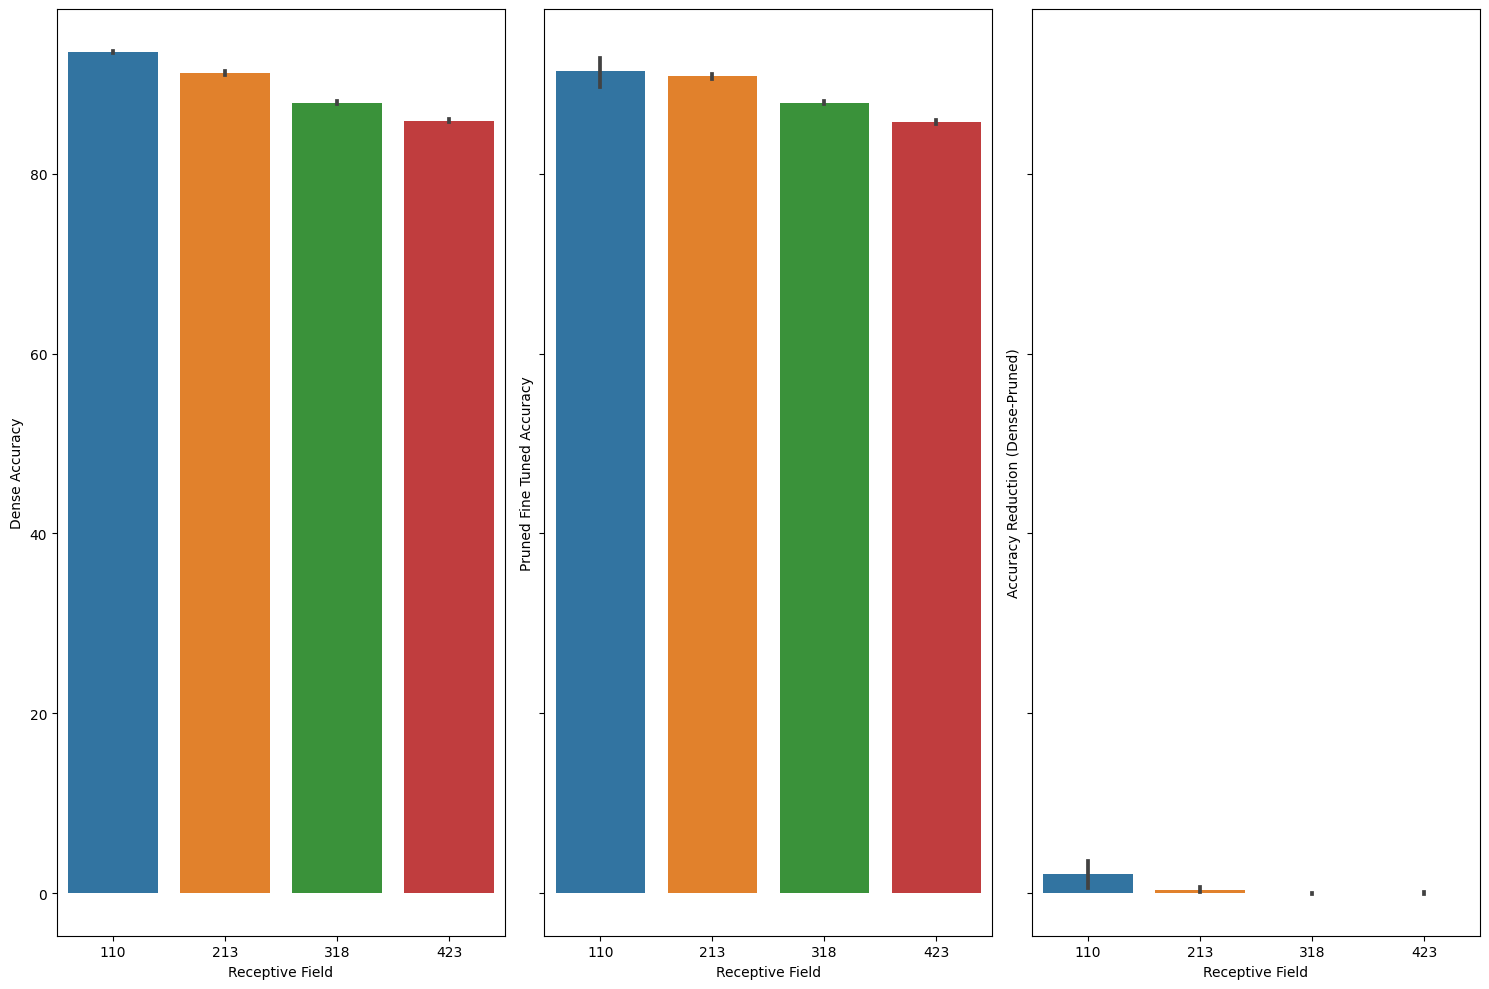
\includegraphics[width=1.1\columnwidth]{images/Supplementary_material/cifar10_vgg19_pruning_finetuned_results_0.9.png}
%    \caption{VGG}
%    \label{subfig:vgg19CIfar10FInetuned}
%     \end{subfigure}
%      \hfill
%     \begin{subfigure}[b]{\columnwidth}
%    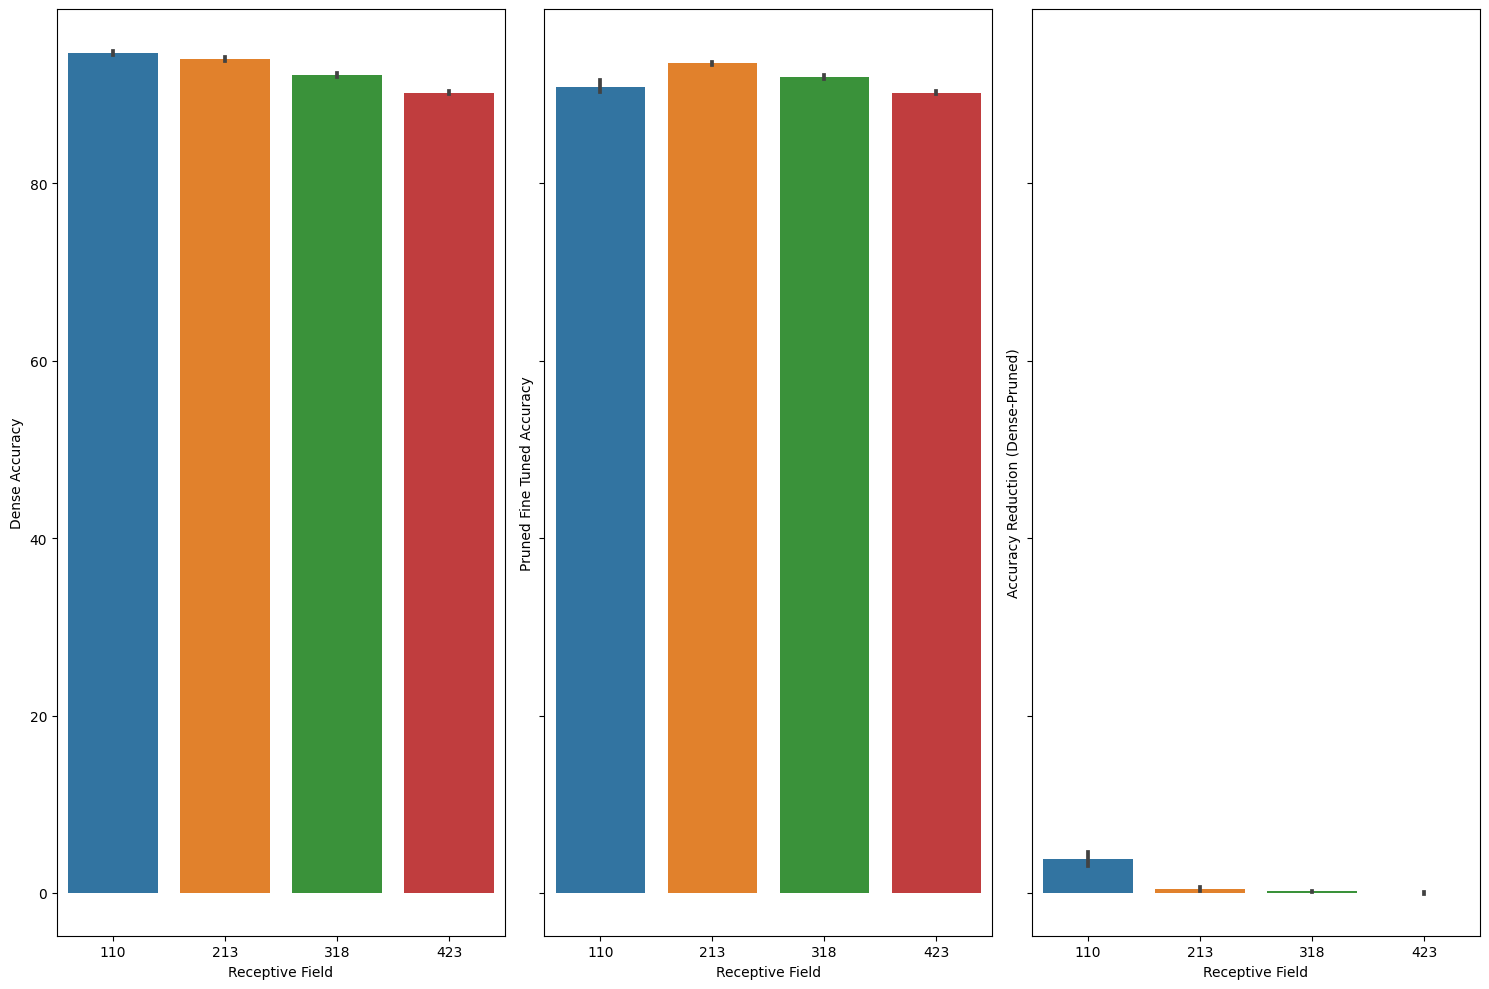
\includegraphics[width=1.1\columnwidth]{images/Supplementary_material/cifar10_resnet50_pruning_finetuned_results_0.9.png}
%    \caption{ResNet-50}
%    \label{subfig:resenet50CIfar10FInetuned}
%     \end{subfigure}
%     \caption{ CIFAR10 Fine-tuned results}
%    \label{fig:finetuned_CIFAR10}
%  \end{figure}
%
%\begin{figure*}[!htb]
% \centering
%     \begin{subfigure}[b]{\columnwidth}
%    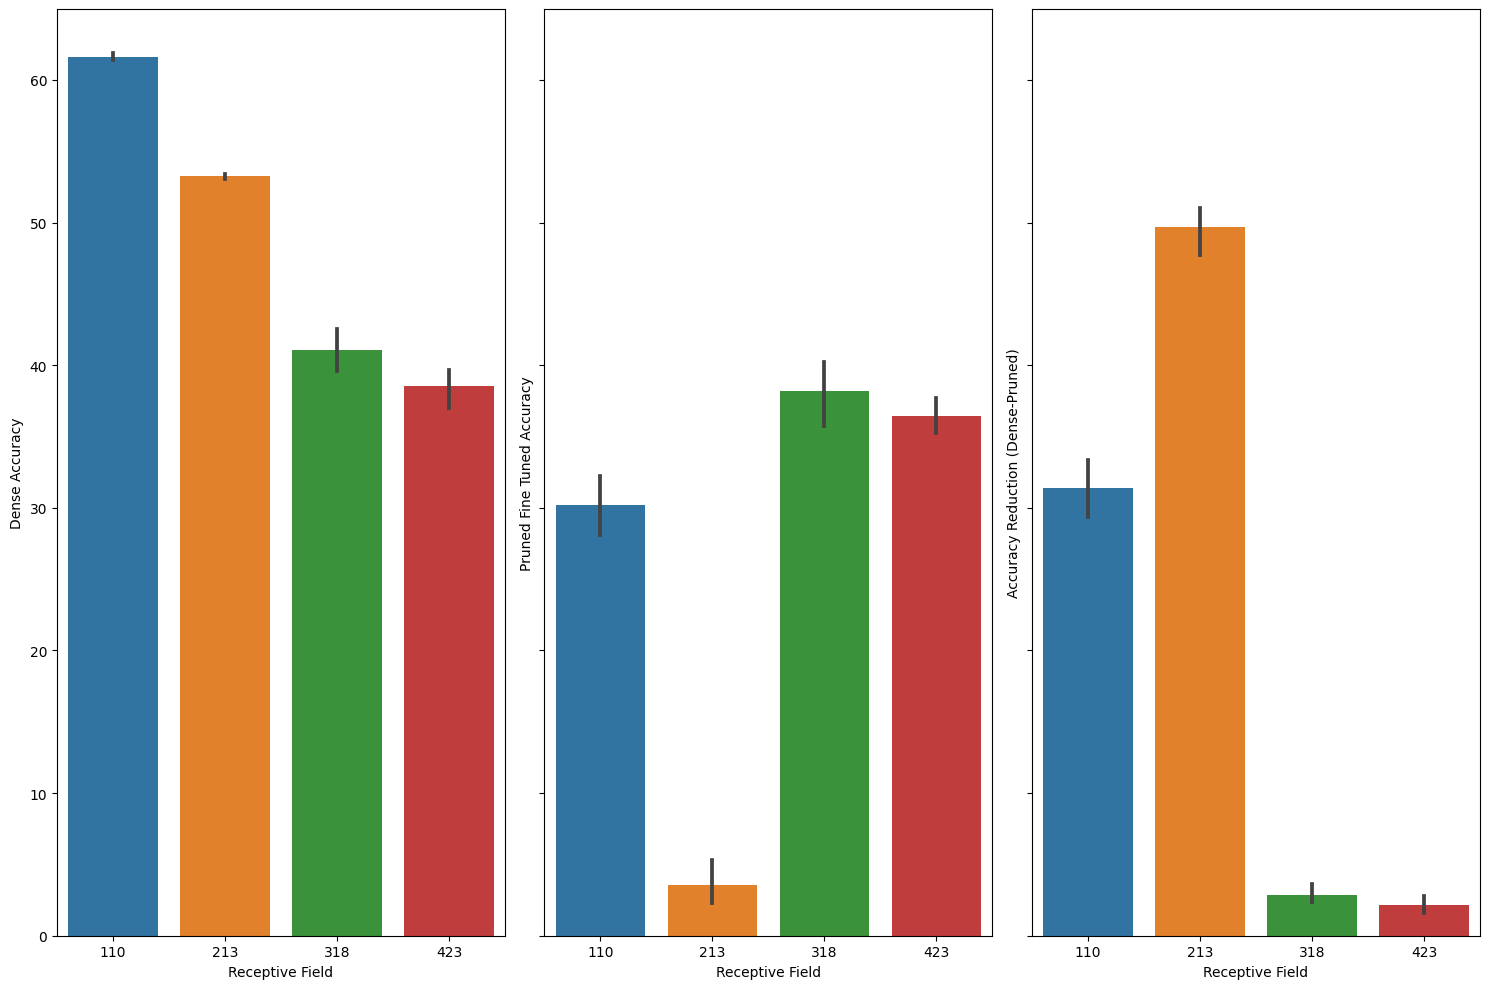
\includegraphics[width=1.1\columnwidth]{images/Supplementary_material/tiny_imagenet_vgg19_pruning_finetuned_results_0.9.png}
%    \caption{VGG}
%    \label{subfig:vgg19_tiny_imagenet_FInetuned}
%     \end{subfigure}
%      \hfill
%     \begin{subfigure}[b]{\columnwidth}
%    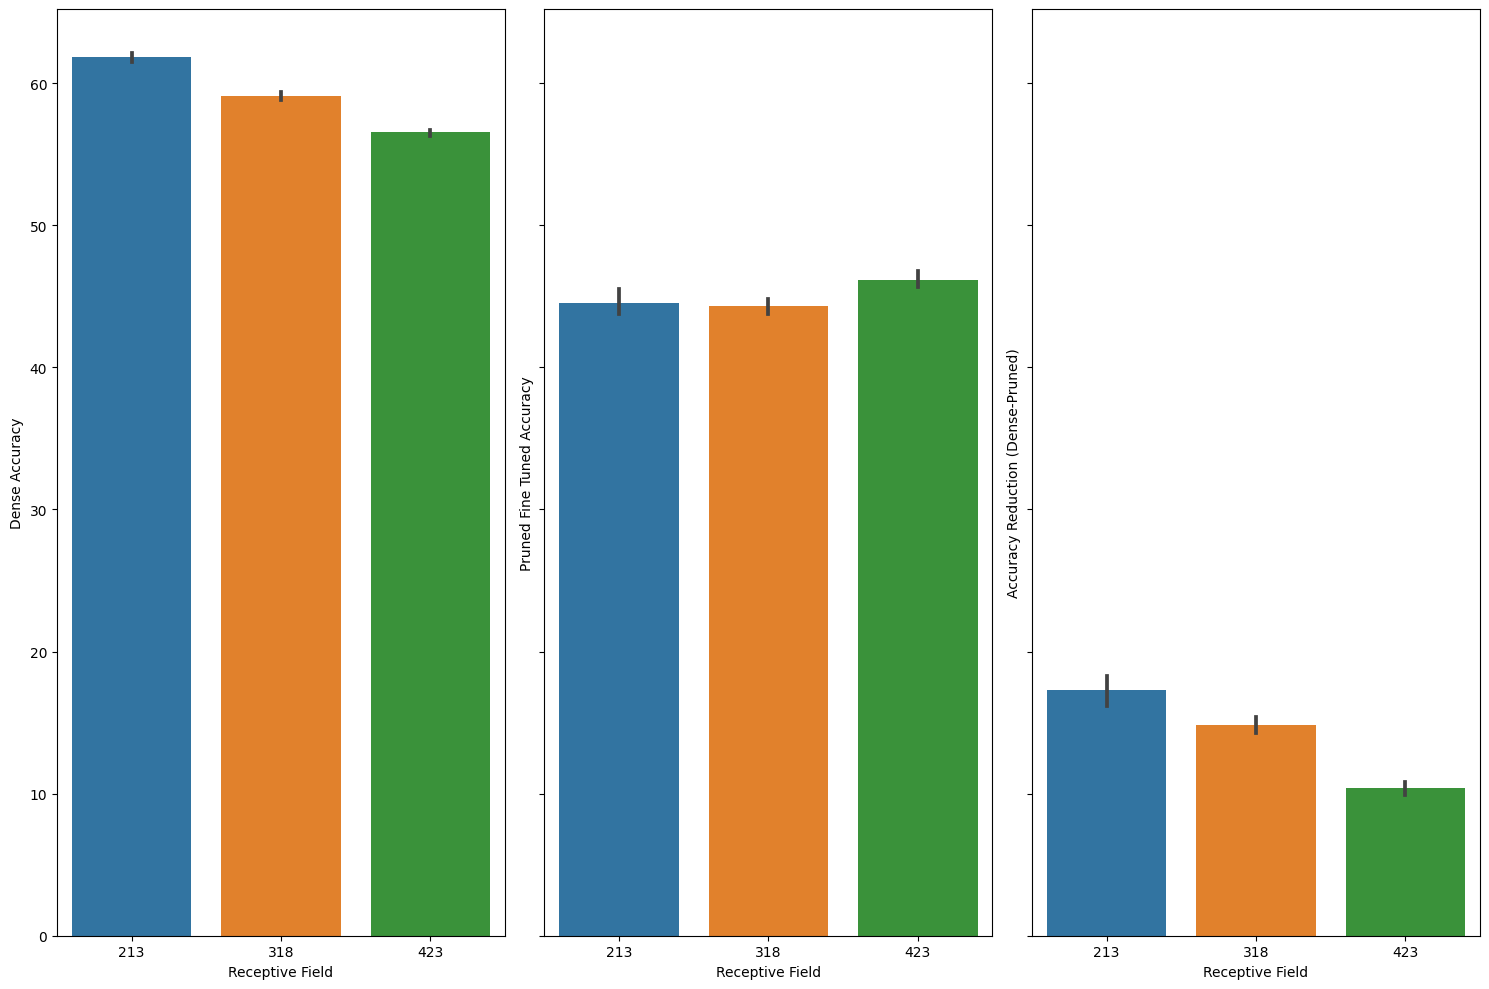
\includegraphics[width=1.1\columnwidth]{images/Supplementary_material/tiny_imagenet_resnet50_pruning_finetuned_results_0.9.png}
%    \caption{ResNet-50}
%    \label{subfig:resenet50tiny_imagenetFinetuned}
%     \end{subfigure}
%     \caption{Tiny ImageNet Fine-tuned results}
%    \label{fig:finetuned_tiny_imagenet}
%\end{figure*}
